\section{Main sequence}\label{sec:main-sequence}
\subsection{Zero-Age Main Sequence}
Dopo aver raggiunto le condizioni adatte per innescare le reazioni termonucleari, la stella comincia la parte più lunga della sua vita, detta Main Sequence (o MS), in cui brucerà idrogeno producendo elio ed energia. Sul piano H-R il punto iniziale della MS per una stella giace sula Zero-Age Main Sequence (in breve ZAMS), una traccia che descrive la luminosità di stelle con la stessa composizione chimica, ma massa differente.

Non tutte le protostelle riescono ad accedere a questa parte dell'evoluzione stellare, infatti, esistono dei limiti al valore che la massa può avere. Data una protostella di massa superiore a $90 \si{solarmass}$, la pressione di radiazione è così elevata che sovrasta quella gravitazionale disperdendo le parti più esterne, per stelle con metallicità molto bassa questo limite può raggiungere anche le $300 - 500 \si{\solarmass}$ così come accadeva per le prime stelle. Nel caso in cui, invece, la massa è inferiore alle $0.08 \si{solarmass}$ allora le temperature nel core non sono abbastanza alte da permettere l'attivazione delle reazioni termonucleari.

\begin{figure}
    \centering
    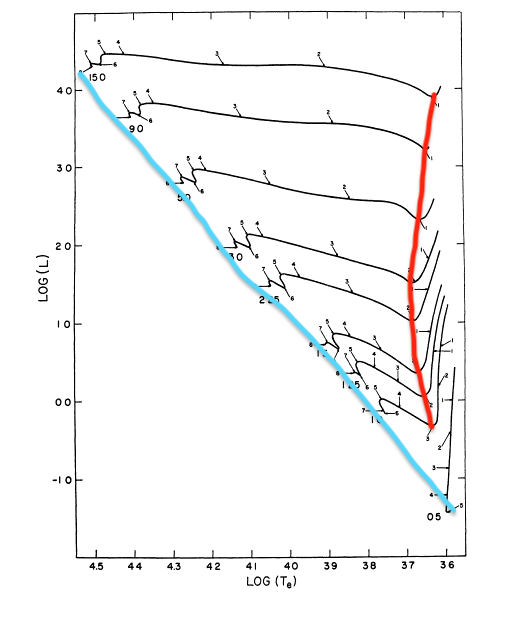
\includegraphics[width = 0.5\textwidth]{immagini/ZAMS.png}
    \caption{La figura mostra la Zero-Age Main Sequence in rosso e la traccia di Hayaschi in azzurro.}\label{fig:ZAMS}
\end{figure}

\subsection{Produzione e trasmissione di energia}\label{sec:prod-tras-energia}

La natura dei meccanismi di fusione influisce anche sull'andamento della luminosità sulla ZAMS, in particolare per stelle molto massive, si ha un andamento che va come $L \propto M^{3.6}$, per quelle relativamente più leggere si ha che $L \propto 4$.  Stelle più piccole hanno infatti temperature del core relativamente più basse rispetto alle stelle più pesanti privilegiando le reazioni a catena PP, che avvengono a temperature di circa $T_e = \SI{1.4e7}{K}$, piuttosto che la CNO, che avvengono nelle in corpi più pesanti, con temperature del nucleo di circa $T_e = \SI{1.8e7}{K}$. Il punto di passaggio tra i due tipi di reazione è molto piccolo e si trova a luminosità di circa $L = 1.2 \si{\solarmass}$.

Il metodo di bruciare il proprio combustibile ha anche delle implicazioni sulla struttura interna della stella, in particolare implica la presenza o meno di convezione negli strati della struttura stellare. Distinguiamo tre possibilità a seconda della posizione che una stella assume sulla ZAMS\: se la massa è inferiore a $0.3 \si{\solarmass}$ allora la struttura sarà completamente convettiva, se la massa è compresa tra le $1.2 \si{\solarmass}$ e le $0.3 \si{\solarmass}$ allora il core avrà una natura radiativa e gli strati più esterni convettivi, mentre per stelle più pesanti di $1.2 \si{\solarmass}$ la situazione è invertita con il core convettivo e gli strati esterni radiativi. Il motivo di queste differenza risiede nel fatto che, nonostante le temperature variano poco, i meccanismi per generare energia sono profondamente diversi. Come visto nella sezione-\ref{sec:catena-pp}

\[
    \epsilon_{\mbox{\footnotesize{pp}}} \propto \rho X^2 T^5
\]
\[
    \epsilon_{\mbox{\footnotesize{CNO}}} \propto \rho X Z_{\mbox{\footnotesize{CNO}}} T^{15}
\]

Per cui si ha che, per masse superiori a $1.2 \si{\solarmass}$, $\epsilon_{\mbox{\footnotesize{pp}}} \ll \epsilon_{\mbox{\footnotesize{CNO}}}$ conseguentemente se la temperatura aumenta, lo farà anche la produzione di energia, assieme alla luminosità. Da quanto visto precedentemente l'aumento di luminosità implica un flusso più intenso, per cui diventa necessario dissipare questa energia più velocemente, si attivano perciò i processi convettivi. Se infatti il flusso aumenta allora aumenta anche il gradiente radiativo e nel momento in cui $\nabla_{rad} > \nabla_{ad}$ si ha convezione nel nucleo.

Per stelle con massa inferiore alle $0.3 \si{\solarmass}$, invece, la totale natura convettiva deriva dal fatto che, per luminosità così basse, la ZAMS coincide con la traccia di Hayaschi.

Nel caso intermedio, infine, la natura radiativa del core è dovuta al fatto che le temperature non sono abbastanza elevate ad innescare le \textit{catene CNO}, per cui la produzione di energia non è intensa come per le loro controparti più massive. La cosa peculiare per queste stelle, però, è la presenza di convezione nella zona esterna della sua struttura, sicuramente non dovuta alle elevate temperature. La spiegazione arriva dall'alta opacità di questi strati, infatti per

\[
    \kappa \propto T^{-3.5}
\]

Al diminuire della temperatura l'opacità aumenta e di conseguenza lo fa anche il gradiente radiativo, fino a che $\nabla_{rad} > \nabla_{ad}$ condizione in per cui si attiva la convezione in quegli strati.

\subsection{Main Sequence}\label{sec:main-sequence-sub}

Dalla ZAMS l'evoluzione stellare entra nella vera e propria main sequence, nella quale fonderà l'idrogeno in elio, modificando molto lentamente la propria composizione chimica. In questa parte della propria vita la stella si trova in uno stato di estrema stabilità, dovuta al fatto che la fusione d'idrogeno è il processo termonucleare più efficiente che esista, motivo per cui questa fase è anche quella più lunga. Ciò nonostante la effettiva durata è variabile della massa iniziale, in particolare il tempo che questa impiega nella MS è inversamente proporzionale alla sua massa iniziale secondo la relazione 
\[
    t_{MS} \cong 10^{10}M^{-3}\mbox{ \footnotesize{(yr)}}
\]
Nella tabella~\ref{tab:MS} è mostrata la durata in anni della main sequence insieme alla massa iniziale, normalizzata a quella solare.
\begin{table}
    \centering
    \caption{Nella tabella sono riportati i valori della durata della main sequence in funzione dei valori della massa stellare, per un campione di stelle.}\label{tab:MS}
    \begin{tabular}{c|ccccccc}
        \toprule
        M [$\si{\solarmass}$] & 15.0 & 9.00 & 5.00 & 3.00 & 2.25 & 1.50 & 1.00\\
        \midrule
        $t_{MS}$ [yr] & $1 \times 10^7$ & $ 2.2 \times 10^7$ & $7 \times 10^7$ & $2\times 10^8$ & $5\times 10^8$ & $1.7 \times 10^9$ & $9\times 10^9$\\
        \bottomrule
    \end{tabular}
\end{table}

Si osserva che data una stella di circe $0.8 \si{\solarmass}$, la durata della sua MS ha lo stesso ordine di grandezza dell'età dell'universo ($t_{MS} \sim 13.9\times 10^9 \mbox{ yr}$). Questo vuol dire che stelle con massa inferiore ad essa e nate poco tempo dopo l'origine dell'universo, saranno ancora nel pieno della propria main sequence.